\documentclass[tikz,border=10pt]{standalone}
\usepackage{amsmath}
\usetikzlibrary{arrows.meta}

\begin{document}
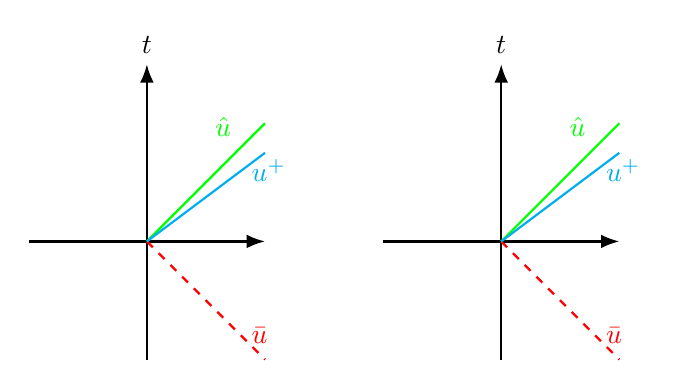
\begin{tikzpicture}[scale=1.5]

% Left Diagram
\draw[-Latex, thick] (-1,0) -- (1,0) node[right] {}; % Horizontal axis (not labeled)
\draw[-Latex, thick] (0,-1) -- (0,1.5) node[above] {$t$}; % Vertical axis

% Wave fronts
\draw[red, dashed, thick] (0,0) -- (1,-1) node[pos=0.8, right] {$\bar{u}$}; % \bar{u}
\draw[green, thick] (0,0) -- (1,1) node[pos=0.8, above left] {$\hat{u}$}; % \hat{u}
\draw[cyan, thick] (0,0) -- (1,0.75) node[pos=0.8, right] {$u^+$}; % u^+

% Right Diagram
\begin{scope}[shift={(3,0)}]
    \draw[-Latex, thick] (-1,0) -- (1,0) node[right] {}; % Horizontal axis (not labeled)
    \draw[-Latex, thick] (0,-1) -- (0,1.5) node[above] {$t$}; % Vertical axis

    % Wave fronts
    \draw[red, dashed, thick] (0,0) -- (1,-1) node[pos=0.8, right] {$\bar{u}$}; % \bar{u}
    \draw[green, thick] (0,0) -- (1,1) node[pos=0.8, above left] {$\hat{u}$}; % \hat{u}
    \draw[cyan, thick] (0,0) -- (1,0.75) node[pos=0.8, right] {$u^+$}; % u^+
\end{scope}
\end{tikzpicture}
\end{document}